\documentclass{beamer}
%
% Choose how your presentation looks.
%
% For more themes, color themes and font themes, see:
% http://deic.uab.es/~iblanes/beamer_gallery/index_by_theme.html
%
\mode<presentation>
{
  \usetheme{Boadilla}      % or try Darmstadt, Madrid, Warsaw, ...
  \usecolortheme{beaver} % or try albatross, beaver, crane, ...
  \usefonttheme{default}  % or try serif, structurebold, ...
  \setbeamertemplate{navigation symbols}{}
  \setbeamertemplate{caption}[numbered]
  
} 

\usepackage{xcolor,colortbl}
\usepackage[english]{babel}
\usepackage[utf8x]{inputenc}
\usepackage{courier}
\usepackage{dsfont}
\usepackage{verbatim} 
\usepackage{enumerate}
\usepackage{tikz}
\usepackage{multirow}
\usepackage{venndiagram}
\usepackage{epigraph} 
%\usepackage{xcolor}
\usepackage{makecell}

%\usepackage{enumitem}

\usepackage{hyperref}
\hypersetup{
    colorlinks=true,
    linkcolor=blue,
    filecolor=magenta,      
    urlcolor=cyan,
}

% R stuff!
\usepackage{listings}
\definecolor{codegreen}{rgb}{0,0.6,0}
\definecolor{codegray}{rgb}{0.5,0.5,0.5}
\definecolor{codepurple}{rgb}{0.58,0,0.82}
\definecolor{backcolour}{rgb}{0.95,0.95,0.92}

\lstdefinestyle{mystyle}{
    backgroundcolor=\color{backcolour},    
    commentstyle=\color{codegreen},
    keywordstyle=\color{black},
    numberstyle=\tiny\color{codegray},
    stringstyle=\color{codepurple},
    basicstyle=\ttfamily\footnotesize,
    breakatwhitespace=false,         
    breaklines=true,                 
    captionpos=b,                    
    keepspaces=true,                 
    numbers=left,                    
    numbersep=5pt,                  
    showspaces=false,                
    showstringspaces=false,
    showtabs=false,                  
    tabsize=2
}

\lstset{style=mystyle}


\setbeamertemplate{enumerate items}[default]
\setbeamertemplate{itemize item}[triangle]

%\setitemize{label=\usebeamerfont*{itemize item}%
%  \usebeamercolor[fg]{itemize item}
%  \usebeamertemplate{itemize item}}



\title[STAT-209]{Confidence Intervals}
\subtitle{Conditions, t-distribution, Different Confidence \%'s}
\author{Grinnell College}
\date{October 18, 2024}

\graphicspath{{img/}}

\begin{document}

\begin{frame}
  \titlepage
\end{frame}

\begin{frame}{Review -- Confidence Intervals}
We learned how to make a "95\% Confidence Interval" for estimating a population mean $\mu$
\begin{align*}
\overline{x} \pm 2 \times \frac{\sigma}{\sqrt{n}}
\end{align*}
\begin{itemize}
    \item 95\% came from the fact that 95\% of the intervals will contain $\mu$
\end{itemize} \vspace{12mm}

\textbf{Intuition:} Think of the confidence interval as providing a range of 'plausible' values for $\mu$
\end{frame}

\begin{frame}{Review -- Central Limit Theorem}
Central Limit Theorem:
\begin{enumerate}
    \item If variable X has mean $\mu$ and std.dev. $\sigma$, and
    \item If the number of observations in the sample (n) is large
    \item then the sampling distribution for $\overline{X}$ (sample mean) is Normal with mean $\mu$ and standard error $\sigma / \sqrt{n}$.
\end{enumerate}
\begin{center}
    $\overline{X} \sim$ N($\mu$, $\sigma / \sqrt{n}$)
\end{center}
\end{frame}

\begin{frame}{More on CLT}
\begin{center}
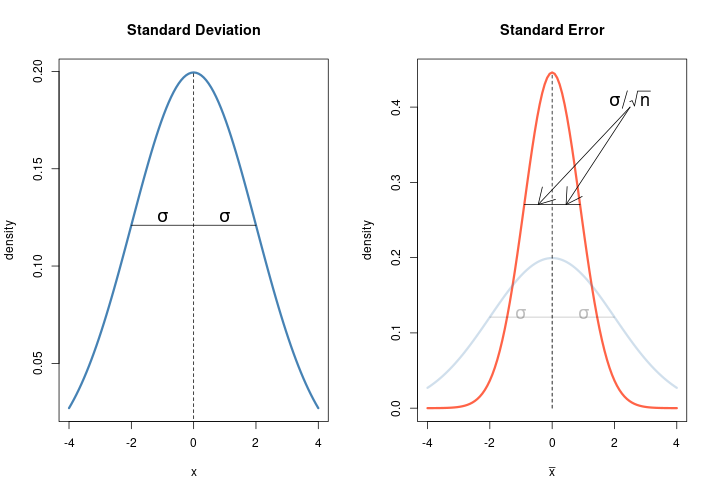
\includegraphics[scale=.4]{sd_vs_se.png}
\end{center}
\end{frame}

\begin{frame}{CI's using Normal Distribution}
Think back to what we were doing with the normal distribution to make our 95\% CI's
\begin{center}
    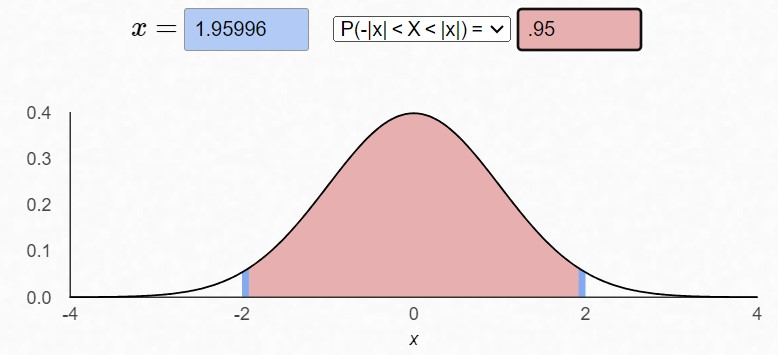
\includegraphics[scale=.7]{img/normal_95ci.jpg}
\end{center}
\textbf{Note:} I lied about using $\pm 2 \times$SE, we actually should be using $\pm 1.96 \times$SE   
\end{frame}

\begin{frame}{CI's using Normal Distribution}
\begin{center}
    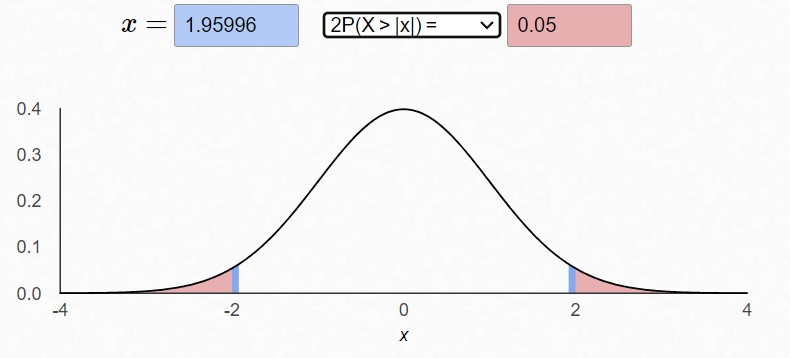
\includegraphics[scale=.6]{img/normal_95ci2.jpg}
\end{center}
\scriptsize
We could find the value we want to use for the ME = $\pm C \times$SE using R
\begin{itemize}
    \item We want 95\% of cases within the values
    \item equivalent we want 5\% outside the values
    \item cut that 5\% in half (2.5\%) to get how much probability we need on each side of the normal distribution
\end{itemize}
\end{frame}

\begin{frame}{qnorm() in R}
\begin{center}
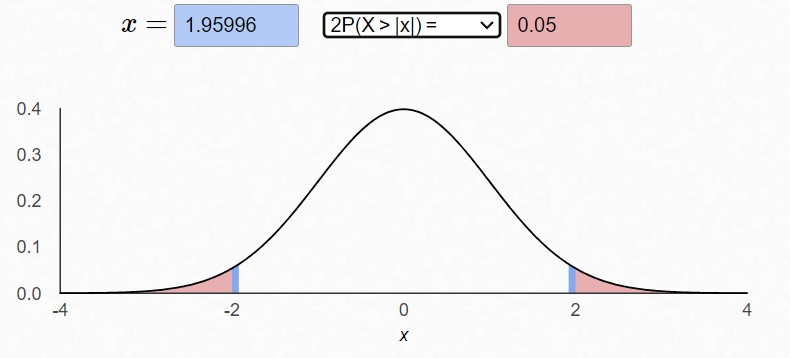
\includegraphics[scale=.5]{img/normal_95ci2.jpg}
\end{center}
\scriptsize
\texttt{pnorm()} let us find probabilities associated with specific values in R
 \vspace{1mm}
 
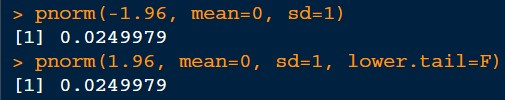
\includegraphics[scale=.9]{img/pnorm.jpg} \vspace{4mm}

\texttt{qnorm()} is a function that does the opposite
\begin{itemize}
    \item gives values that correspond to specific probabilities
\end{itemize}
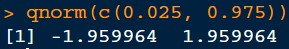
\includegraphics[scale=.9]{img/qnorm1.jpg}

\end{frame}

\begin{frame}{Another Issue}
\textbf{95 \% CI Formula ($\sigma$ known):}
\begin{align*}
\overline{x} \pm 1.96 \times \frac{\sigma}{\sqrt{n}}
\end{align*} \vspace{10mm}

We don't know $\mu$, which is why we are trying to estimate it. \vspace{2mm}

Do we know $\sigma$? Probably not! Let's try... \vspace{10mm}

\textbf{95 \% CI Formula ($\sigma$ unknown):}
\begin{align*}
\overline{x} \pm 1.96 \times \frac{s}{\sqrt{n}}
\end{align*}
\end{frame}

\begin{frame}{Conditions}
When we don't know the value of $\sigma$... \vspace{15mm}

We need at least one of these things to be true in order for our 95\% CI formula to work (CLT)
\begin{itemize}
    \item The \textit{population} must be Normal
        \begin{itemize}
            \item we will almost always never know if this is true
        \end{itemize}
    \item sample size n $\geq$ 30
\end{itemize}
\end{frame}

\begin{frame}{Conditions}
\scriptsize \hspace{15mm} N = 50 \vspace{-1mm}
\begin{center}
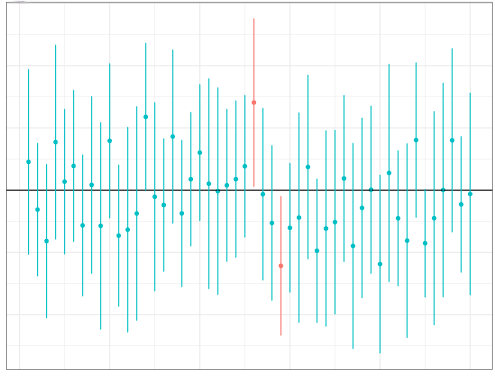
\includegraphics[scale=0.68]{n50.png}
\end{center}
\end{frame}

\begin{frame}{Conditions}
\begin{center}
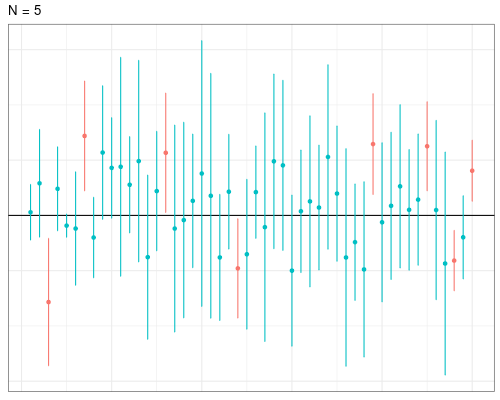
\includegraphics[scale=0.5]{n5.png}
\end{center}
\end{frame}

\begin{frame}{Conditions}
We need the following to be true in order for our 95\% CI formula to work (CLT)
\begin{itemize}
    \item random sample
    \item sample size n $\geq$ 30
\end{itemize} \vspace{10mm}

Why?
\begin{itemize}
    \item Without these, the sampling distribution is not close enough to Normal (or is biased)
    \item Our intervals contain $\mu$ less than 95\% of the time
\end{itemize}
\end{frame}


\begin{frame}{Estimating Variance}
Sampling Distribution of the sampling mean:
\begin{align*}
\overline{X} \sim N \left( \mu, \ \frac{\sigma}{\sqrt{n}} \right)
\end{align*}

\begin{itemize}
\item The sampling distribution depends on $\sigma$, not \textbf{s}
\item Is \textbf{s} going to be exactly equal to $\sigma$? NO!
\end{itemize}

\vspace{15mm}
There is uncertainty in estimating $\sigma$ using \textbf{s} just like how we are using $\overline{x}$ to estimate $\mu$
\begin{itemize}
    \item We need a way to incorporate our uncertainty about $\sigma$ into the confidence intervals we construct for $\overline{x}$
\end{itemize}
\end{frame}

\begin{frame}{Student's $t$-distribution}
\small
In the 1890s, a chemist by the name of William Gosset working for Guinness Brewing became aware of the issue while investigating yields for different barley strains \vspace{3mm}

In 1906, he took a leave of absence to study under Karl Pearson where he discovered the issue to be the use of $\hat{\sigma}$ with $\sigma$ interchangeably  \vspace{3mm}

To account for the additional uncertainty in using $\hat{\sigma}$ as a substitute, he introduced a modified distribution that has ``fatter tails" than the standard normal \vspace{3mm}

However, because Guinness was not keen on its competitors finding out that it was hiring statisticians, he was forced to publish his new distribution under the pseudonym "student", hence ``Student's $t$-distribution"

\end{frame}

\begin{frame}{Student's $t$-distribution}
Student's $t$ Distribution:
\begin{align*}
X \sim t(n-1)
\end{align*}

\begin{enumerate}
\item symmetric around zero
\item bell-shaped
\item one parameter called the \textit{degrees of freedom}, equal to $n-1$
\item has more probability in the tails than the normal distribution
\item The $t$ distribution will become normal as $n \rightarrow \infty$
\end{enumerate}
\end{frame}

\begin{frame}{t-distribution with df=3}
\begin{center}
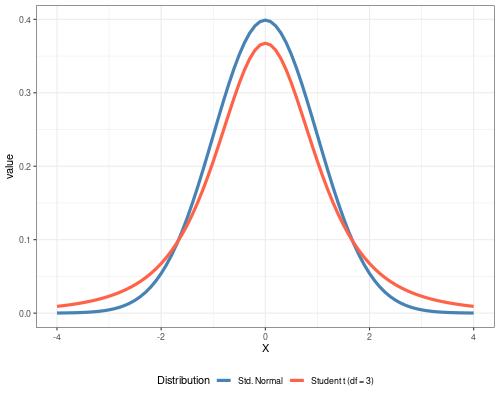
\includegraphics[scale=0.5]{t3.png}
\end{center}
\end{frame}

\begin{frame}{t-distribution with df=10}
\begin{center}
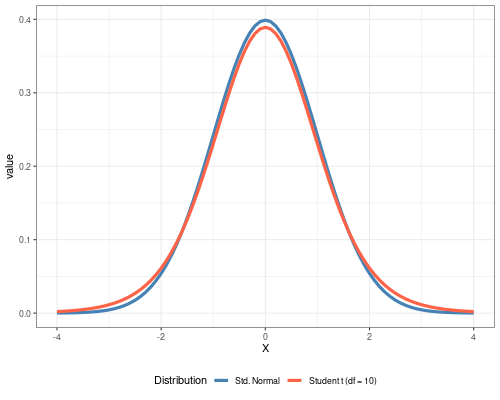
\includegraphics[scale=0.5]{t10.png}
\end{center}
\end{frame}

\begin{frame}{t-distribution with df=29}
\begin{center}
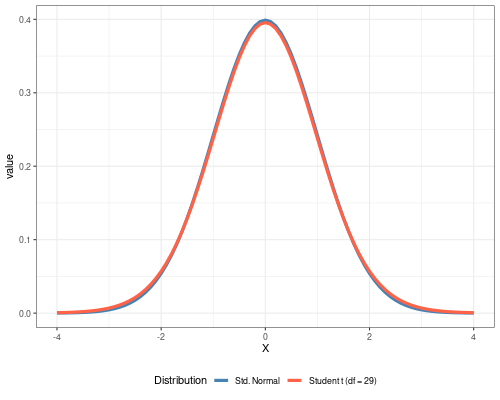
\includegraphics[scale=0.5]{t30.png}
\end{center}
\end{frame}

\begin{frame}{Implications?}
What are the implications of this for our confidence intervals? \vspace{4mm}

\begin{center}
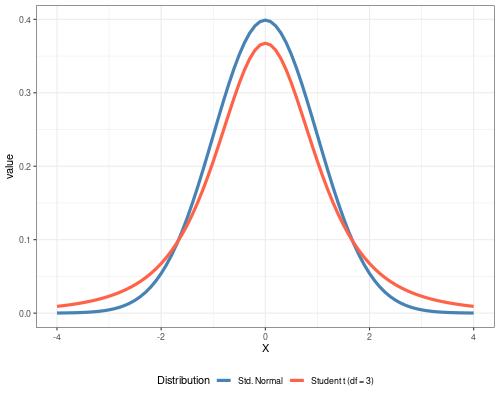
\includegraphics[scale=0.4]{t3.png}
\end{center}
\begin{itemize}
    \item we can't just use $\pm 1.96 \times$SE
    \item we need to go out further because there is more probability in the tails
\end{itemize}
\end{frame}

\begin{frame}{CI's using t-distribution}
How do we go about making 95\% CI's for the t-distribution?
\begin{center}
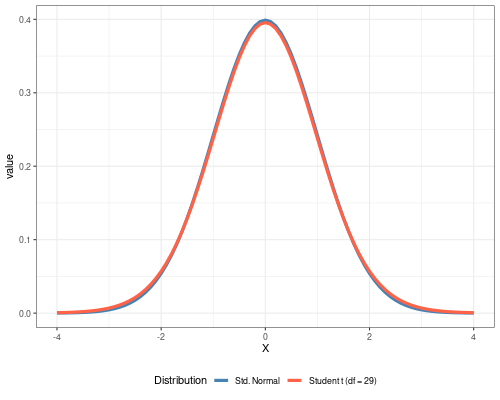
\includegraphics[scale=0.4]{t30.png}

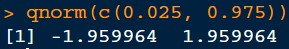
\includegraphics[scale=.9]{img/qnorm1.jpg}
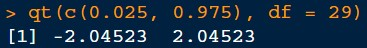
\includegraphics[scale=.9]{img/qnorm2.jpg}
\end{center}
\end{frame}

\begin{frame}{CI's using t-distribution}
How do we go about making 95\% CI's for the t-distribution?
\begin{center}
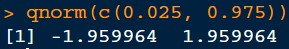
\includegraphics[scale=.9]{img/qnorm1.jpg}
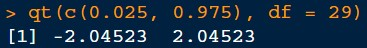
\includegraphics[scale=.9]{img/qnorm2.jpg}
\end{center}

Instead of using:

\begin{align*}
\overline{x} \pm 1.96 \times \frac{s}{\sqrt{n}},
\end{align*}

We will use:
\begin{align*}
\overline{x} \pm t_{(.975, df=n-1)} \times \frac{s}{\sqrt{n}},
\end{align*}
\begin{itemize}
    \item $t_{(.975, df=n-1)}$ is the value corresponding to the .975 quantile of a t-distribution using df=n-1
    \item we use \texttt{qt(.975, df = n - 1)} in R to get this value
\end{itemize}
\end{frame}

\begin{frame}{Comparing CI's between Normal and t-dist}
\begin{center}
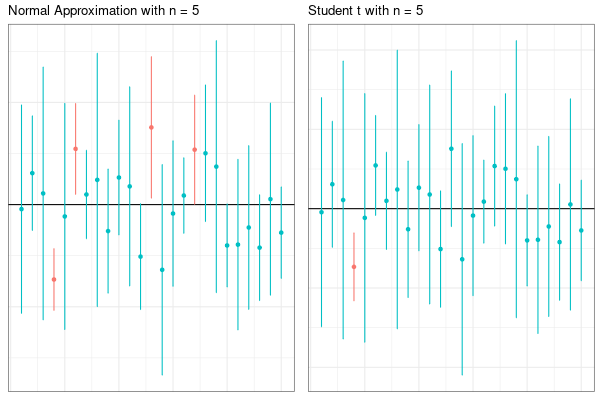
\includegraphics[scale=0.5]{norm_vs_t.png}
\end{center}
\end{frame}

\begin{frame}{Different \% CI's}
We may not always want a 95\% confidence interval
\begin{itemize}
    \item maybe we are OK with an 80\% CI
    \item maybe we want a 99\% CI
    \item remember that there is a trade-off between confidence \% and how wide the interval is
\end{itemize} \vspace{10mm}

What do we do? We just adjust the margin of error to account for the new confidence \% we want.
\end{frame}

\begin{frame}{Different \% CIs}
\scriptsize{
Let $\alpha$ denote the \% of confidence intervals that will incorrectly estimate $\mu$ (as a decimal)
\begin{itemize}
    \item then we can say we are trying to find a 100(1-$\alpha$)\% CI
    \item ex) for a 95\% CI, we have $\alpha = .05$
    \item ex) for a 80\% CI, we have $\alpha = .2$
\end{itemize} \vspace{6mm}

To find the associated cutoffs on the t-distribution for a 100(1-$\alpha$)\% CI:
\begin{itemize}
    \item calculate $\alpha$ value
    \item use qt() function in R
    \item the appropriate value to put in the funtion is ($1-\frac{\alpha}{2}$)
\end{itemize}} \vspace{4mm}

\textbf{General Formula} for 100(1-$\alpha$)\% CI
\begin{align*}
\overline{x} \pm t_{(1-\frac{\alpha}{2}, df=n-1)} \times \frac{s}{\sqrt{n}},
\end{align*}
\end{frame}

%%%%%%%%%%%%%%%%

%\begin{frame}
%\begin{columns}
%
%  \begin{column}{0.45\textwidth}
%%
%  \end{column}
%  \begin{column}{0.45\textwidth}
%%
%  \end{column}
%
%\end{columns}
%\end{frame}


\end{document}
